\documentclass[FM,DP]{tulthesis}

\usepackage{polyglossia}
\setdefaultlanguage{czech}
\usepackage{fontspec}
\usepackage{xunicode}
\usepackage{xltxtra}
\setsansfont[Mapping=tex-text,BoldFont={* Bold},Numbers=OldStyle]{Myriad Pro}
\usepackage{hyperref}
\hypersetup{colorlinks=true, linkcolor=tul, urlcolor=tul, citecolor=tul}
\usepackage{graphicx}
\usepackage{listings}
\usepackage[toc,page]{appendix}
\usepackage{amsmath}
\usepackage{amssymb}
\newcommand{\argument}[1]{{\ttfamily\color{\tulcolor}#1}}
\newcommand{\prikaz}[1]{\argument{\textbackslash #1}}
\newenvironment{myquote}{\begin{list}{}{\setlength\leftmargin\parindent}\item[]}{\end{list}}
\newenvironment{listing}{\begin{myquote}\color{\tulcolor}}{\end{myquote}}
\sloppy


%%%%%%%%%%%%%%%%%%%%%%%%%%%%
\TULtitle{Vyhledávání jako služba}{Search as a Service}
\TULprogramme{Aplikovaná informatika}{Applied Informatics}
\TULbranch{Informační systémy a technologie}{Information Technologies}
\TULauthor{Bc. Luděk Veselý}
\TULsupervisor{Prof. Ing. Zdeněk Molnár, CSc.}
\TULyear{2017}


%%%%%%%%%%%%%%%%%%%%%%%%%%%%
\begin{document}
\ThesisStart{male}


%%%%%%%%%%%%%%%%%%%%%%%%%%%%
\begin{abstractCZ}
Tato diplomová práce popisuje návrh a tvorbu fulltextového vyhledávání poskytovaného jako služba.
\end{abstractCZ}

\begin{klicovaslovaCZ}
Fulltext, Elasticsearch
\end{klicovaslovaCZ}

\vspace{2cm}

\begin{abstractEN}
This diploma thesis describes creation of fulltext search service.
\end{abstractEN}

\begin{klicovaslovaEN}
Fulltext, Elasticsearch
\end{klicovaslovaEN}


%%%%%%%%%%%%%%%%%%%%%%%%%%%%
\begin{acknowledgement}
Rád bych poděkoval Ing. Ivanovi Jelínkovi za rady a pomoc při řešení.
\end{acknowledgement}


%%%%%%%%%%%%%%%%%%%%%%%%%%%%
\tableofcontents
\clearpage


%%%%%%%%%%%%%%%%%%%%%%%%%%%%
%\begin{abbrList}
%\textbf{e-shop} & 
%Elektronický obchod\\
%\end{abbrList}


%%%%%%%%%%%%%%%%%%%%%%%%%%%%
\chapter{Úvod}

V~této diplomové práci práci se zabývám návrhem a implementací nástroje, který umožňuje
provozovatelům elektronických obchodů snadnou a rychlou implementaci plnotextového vyhledávání. 
Při jeho implementaci je totiž třeba mít určitou úroveň znalosti principů samotného 
vyhledávání včetně souvisejících oborů a technologií. Implementace kvalitního vyhledávání
tak může být pro provozovatele elektronického obchodu náročná jak časově, tak finančně.
Tento nástroj je poskytován jako služba se všemi výhodami i omezeními s tímto principem spojenými. 
Konkrétní cíle diplomové práce popisuji v následujících odstavcích.

\section{Cíle práce}

Cílem práce je vytvořit nástroj, který je nabízen jako služba a umožňuje snadnou implementaci
plnotextového vyhledávání do elektronického obchodu. K~dosažení tohoto cíle je třeba naplnit cíle dílčí.

Prvním dílčím cíem je provedení analýzy problému a to jak z~pohledu byznysového, tak
z~pohledu samotné problematiky vyhledávání. Co se týče pohledu byznysového, tak je třeba
analyzovat potřeby zákazníků, zjistit, jaká jsou specifika oblasti elektronického obchodování
a definovat kritéria, jejichž naplnění je pro provozovatele elektronických obchodů klíčové. 
Z~pohledu problematiky vyhledávání je pak třeba provést analýzu této disciplíny a utřídit
tak znalosti potřebné k poskytnutí kvalitních výsledků plnotextového vyhledávání.

Dalším dílčím cílem je vytvořit návrh řešení problému jednak na základě znalosti potřeb
zákazníků a také na základě znalosti problematiky plnotextového vyhledávání. Tento návrh musí 
být v~dalším kroku implementovatelný.

Posledním dílčím cílem je samotná implementace aplikace dle jejího návrhu. Obnáší to výběr 
vhodných nástrojů, jejich nasazení do produkčního prostředí, naprogramování jednotlivých
služeb a konečně také ověření samotné implementace. Tu je třeba porovnat vůči požadavkům
a ověřit tak jejich naplnění.

\section{Cílová skupina}

První cílovou skupinou je vývojář, řešící problém plnotextového vyhledávání produktů 
při implementaci elektronického obchodu. Takovému čtenáři by měla práce poskytnout dostatečné
teoretické znalosti potřebné pro implementaci vyhledávání. Užitečná také může být konkrétní
podoba implementace, která je v této práci popisována.

Další možnou cílovou skupinou je provozovatel elektronického obchodu, který přemýšlí, 
jakým způsobem zlepšit (případně zavést) plnotextové vyhledávání. V~této práci získá 
přehled o~složitosti samotné implementace, poskytne mu komentovaný soupis možných řešení 
a konečně také poskytne funkční službu, kterou může okamžitě na~webový portál napojit.

Poslední cílovou skupinou budiž kdokoli, kdo se zajímá o problematiku plnotextového 
vyhledávání v českém jazyce. V této práci nalezne soupis problémů souvisejicích s češtinou, 
které je třeba řešit. Dále zde nalezne konkrétní implementaci, kterou se může inspirovat 
při řešení obdobného problému.

\section{Použité metody}

V~této části popisuji metody použité k~naplnění jednotlivých cílů. Pro zkoumání problému
oboru provedu analýzu trhu, nabízí se také možnost dotazování potenciálních uživatelů.
Pro porozumnění problematice vyhledávání provedu rešerši literatury. Vzhledem k množství
dostupné literatury bude třeba provést syntézu těchto informací. Při vytváření 
návrhu řešení bude použito modelování, výstupem by tedy měl být model řešení. 

\section{Struktura práce}

V první části práce popisuji problematiku vyhledávání v~prostředí elektronického obchodování. 
Definuji zde jednak kontext, v~kterém se pohybuji a dále také popisuji problémy, 
které v~tomto prostředí existují. Snažím se identifikovat potencionálního uživatele 
a definovat jeho požadavky na~plnotextové vyhledávání. Toto prostředí má svá specifika, 
která také popisuji a vysvětluji, přoč jsem se na tuto oblast zaměřil. V~závěru této části porovnávám
existující nástroje umožňující implementaci vyhledávání a zjišťuji tak, proč má smysl
vytvářet další službu, jaká je její přidaná hodnota.

V druhé části se zabývám teorií plnotextového vyhledávání. Popisuji zde celý
proces od analýzy vstupních dat, přes jejich indexaci, až po samotné vyhledávání. 
Tyto poznatky budou následně využity k~naplnění požadavků na vyhledávání, k~zajištění
kvalitních výsledků vyhledávání.

V další části práce navrhuji samotnou aplikaci tak, aby vyhovovala požadavkům a zároveň byla 
následně implementovatelná. Porovnávám zde dostupné nástroje, definuji přípday užití aplikace
a vytvářím model výsledné aplikace.

V poslední části diplomové práce popisuji konkrétní implementaci v~jazyce Go s~pomocí úložiště 
Elasticsearch. Výstupem této části je otestovaný spustitelný program, který umožňuje provádět 
indexaci produktů a jejich následné vyhledávání.


%%%%%%%%%%%%%%%%%%%%%%%%%%%%
%\chapter{Komentovaná rešerše informačních zdrojů}
%...


%%%%%%%%%%%%%%%%%%%%%%%%%%%%
\chapter{Analýza byznys požadavků na aplikaci}

V první části diplomové práce popisuji problematiku plnotextového vyhledávání 
v~prostředí elektronických obchodů. Nejprve je čtenář uveden do problematiky elektronického
obchodování a obeznámen s základními pojmy a principy. Následně je popsán problém, 
který je řešen a jsou definovány konkrétní podmínky, za kterých bude výsledný nástroj
přínosný a použitelný. Jsou zde také diskutovány stávající možnosti implementace
plnotextového vyhledávání a porovnány alternativní služby.

\section{Vysvětlení základních pojmů}

Pro usnadnění orientace v této práci nejprve vysvětluji dále používané pojmy. Jedná se 
vesměs o známé termíny, přesto považuji za důležité uvést jejich význam na pravou míru.

\subsection*{Elektronické obchodování}

Termín elektronické obchodování (e-commerce) označuje veškerou činnost spojenou s obchodováním
realizovaným prostřednictvím sítě internet \cite[strana~11]{e-commerce}. Spadá sem distribuce, nákup, 
prodej, marketing, servis produktů. Elektronické obchodování se dále podle dělí zaměření na cílové 
skupiny, z nichž nejpodstatnější jsou B2C (zaměřeno na koncové zákazníky) a B2B (zaměřeno na obchodníky) 
\cite[strana~17]{e-commerce}. Zároveň je však elektronické obchodování podmnožinou 
elektronického podnikání (e-business), které oznažuje veškeré obchodní a výrobní aktivity, 
zatímco elektronické obchodování se týká samotného prodeje zboží a služeb.

\subsection*{Elektronický obchod}

Elektronický čí internetový obchod (e-shop) je webová aplikace, jejímž prostřednictvím 
provozovatel obchodu prodává zboží nebo služby zákazníkům \cite[strana~16]{e-commerce}.
Jedná se o podmožinu elektronického obchodování, jde tedy o jeden z možných prodejních 
kanálů v prostředí internetu. Elektronický obchod je specifickou webovou aplikací, v~níž 
se opakují určité vzorce. Konkrétně je to katalog produktů, kategorizace zboží, 
vkládání položek do košíku, platba objednávky, možnost kontaktu s zákaznickou podporou 
prostřednictvím on-line chatu přímo v aplikaci.

V elektronickém obchodě můžeme shledávat řadu podobností s obchodem kamenným, který zákazníci 
navštěvují osobně. Některé vlastnosti elektronického obchodu jsou zřejmě inspirovány 
obchody kamennými (procházení zboží podle kategorií, přidávání položek do košíku, 
uplatnění slevových poukázek při platbě). Často však elektronický obchod využívá možností, 
které webové prostředí nabízí (filtrace a řazení položek podle parametrů, vrácení se
k naplněnému košíku, porovnávání zboží napříč obchody).

\begin{figure}[h]
\center
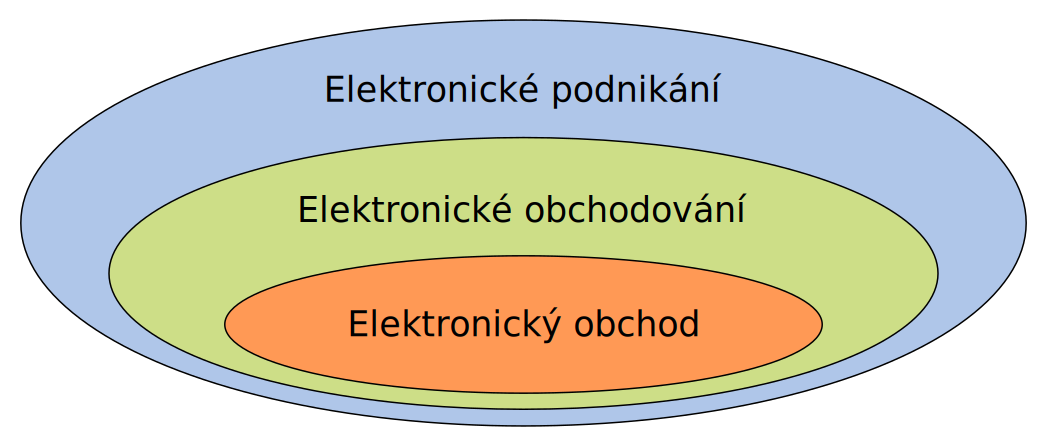
\includegraphics[width=\textwidth]{e-commerce.pdf}
\caption{Vztah elektronického podnikání, obchodování a podnikání}
\label{foto}
\end{figure}

Zcela zásadní výhodou elektronického obchodu oproti návštěvě obchodu kamenného
je možnost vytvoření objednávky z pohodlí domova a její následné doručení zásilkovou 
službou. Tento přístup především šetří čas strávený cestou do obchodu a čas strávený 
v~obchodě. Například v segmentu nákupu potravin může být výhodou to, že je takový 
nákup hygieničtější a zboží bude doručeno v lepším stavu díky uzpůsobeným vozům dopravců.
Výhody ale vznikají i pro provozovatele - nemusí zřizovat prodejnu včetně jejího vybavení a 
zaměstnance, mohou efektivněji navrhnout sklad, nebo dokonce využít automatizace 
při kompletaci objednaného zboží.

\subsection*{Plnotextové vyhledávání}

Plnotextové vyhledávání (full-text search), je způsob vyhledávání v textových datech, 
kdy se vyhledává uživatelem formulovaný dotaz v invertovaném souboru (někdy také 
indexovém souboru nebo invertovaném indexu), tedy v souboru obsahující výrazy, 
podle nichž je daný záznam vyhledatelný \cite[strana~15]{strossa}. 
Proces, kterým vzniká indexový soubor se nazývá indexace. Tato problematika je podrobněji
popisována v druhé kapitole.

\section{Vysvětlení problému, který je řešen}

Plnotextové vyhledávání je rychlým prostředkem nalezení konkrétního produktu
v elektronickém obchodě. Typicky je využito zákazníky, kteří jsou na webu
s konkrétní potřebou a jsou schopni formulovat výraz, podle kterého produkt
hledají. Může jít o název tybu produktu, jeho značku, variantu nebo kategorii.
Pro takového uživatele je procházení webu procházením kategorií zdlouhavé
a právě plnotextové vyhledávání mu může zásadně zrychlit cestu k nalezení 
hledaného produktu.

Důležitost plnotextového vyhledávání navíc roste s rostoucím počtem produktů a kategorií, 
v kterých je složité se orientovat. Uživatel tak může vyhledávání využít už pro 
nalezení kategorie, která se nachází v dlouhém a nepřehledném menu.

\begin{figure}[h]
\center
\includegraphics[width=\textwidth]{atoto-full-text.png}
\caption{Ukázka plnotextového vyhledávání}
\label{foto}
\end{figure}

Implementace plnotextového vyhledávání však není triviální záležitostí. Vstup uživatele
je v přirozeném jazyce, takže je třeba jej odpovídajícím způsobem zpracovat, 
aby bylo vůbec vyhledávání na webu použitelné. Studium této problematiky
může být zdlouhavé a v konečném důsledku drahé. Pokud bude k dispozici hotové řešení, 
které bude snadno nasaditelné na elektronický obchod a bude umožňovat jednoduché 
uzpůsobení potřebám konkrétního webu, bude to výrazná úspora jak času, tak peněz
provozovatele obchodu.

\section{Specifika prostředí elektronického obchodování}

V prostředí elektronického obchodování existují jisté vzorce které se opakují a odlišují
toto prostředí od ostatních. Vyhledávají se zpravidla produkty (případně služby), které jsou
zařazeny do určitých kategorií a disponují atributy jako cena, název, kód, popis, url, obrázek, 
dostupnost a dalšími parametry, které bývají číselné (hmotnost, objem) nebo výčtové (barva, značka). 

Z toho vyplývá co a podle čeho se bude vyhledávat. Produkty mívají jednoznačné identifikátory, 
které jsou navíc standardizovány (EAN, ISBN). Pomocí těchto kódu je možné vyhledat produkty
napříč elektronickými obchody nebo je párovat v cenových srovnávačích. Pro vyhledávání
je dále důležitý název produktu, případně jeho varianty, která upřesňuje konkrétní
verzi produktu. Méně častěji je nutné vyhledávat v popisu produktu, kde bývá uveden
jak slovní popis, tak výpis parametrů. 

U produktů dále bývá evidována cena, která může být interně uložena v kombinaci s marží.
Obchody operující se zlevněným zbožím pak mívají uvedenou cenu jak před slevou, tak po této
slevě, aby zákazník viděl, kolikaprocentní sleva je na produktu. I samotná cena produktu
(případně marže prodejce) může hrát svou roli ve vyhledávání.

\section{Definice požadavků na vyhledávání}

Požadavky na samotné vyhledávání jsou ovlivněny prostředím, ve kterém vyhledávání
probíhá a uživateli, kteří vyhledávání využívají. Primárně by mělo být možné
nalézt daný produkt podle jeho názvu, nebo části názvu. To samé platí pro 
kód produktu. Produkt by měl být ale vyhledatelný i podle dalších atributů, 
jako je název kategorie nebo název značky výrobce. Někdy dokonce uživatel nemusí
vyhledávat konkrétní produkt, ale jen produkty dané značky nebo kategorie, což by
měl systém také umět rozpoznat.

Podoba vyhledávaných výrazů bude zadávána zákazníky v přirozeném jazyce, s čímž by si mělo
vyhledávání také poradit. Konkrétně jde o tvarosloví, kdy může uživatel zadat výraz
například v jiném pádu, než je uvedeno v názvu produktu. Dále jde o vyrovnání se
s~chybami, které mohou vzniknout při formulaci vyhledávaného výrazu - překlepy nebo
pravopisné chyby. V neposlední řadě jde také o vztah slova k jeho významu, kdy může
jedno slovo mít více významů (homonymum) nebo naopak více slov může odpovídat jednomu výrazu
(synonymum).

Další problematikou při zadávání hledaného výrazu uživatelem, je poskytování relevantních výsledků
už ve chvíli, kdy uživatel formuluje dotaz, tedy jej teprve píše. V takovém případě je třeba
odhadnout, který výraz chce napsat a tuto informaci využít při zobrazení odpovídajících
cýsledků.

Ve chvíli, kdy systém zná produkty, které odpovídají hledanému výrazu by měl
výsledky poskytovat ve vhodném pořadí, měl by tedy pracovat s relevancí výsledků vzhledem 
k~zadanému výrazu. Toto může být velmi obtížné, protože každý uživatel má zájem o jiné
produkty a tak pro něj mohou být ro jeden výraz relevantní jiné produkty, než pro někoho
jiného. Dále do tohoto pořadí můžou vstupovat požadavky provozovatele elektronického obchodu
v případě, kdy má specifické požadavky na zboží, které chce nabízet přednostně. Důvodů
pro takové chování může být více, může souviset s marží konkrétních produktů, 
nebo s filozofií samotného obchodu.

\section{Technické požadavky na aplikaci}

Na aplikaci je kladeno několik technických požadavků. Nejedná se o funkční požadavky, nýbrž
o požadavky související s použitelností, výkonností, spolehlivostí a podporou. Naplnění těchto
požadavků zajistí následný bezproblémový chod aplikace a uspokojení potřeb zákazníka.

Prvním technickým požadavkem na aplikaci je její rychlost. Ta je důležitá pro spokojenost
koncového zákazníka, který provádí vyhledávání. Všechny části aplikace nejsou z hlediska rychlosti
tak kritické, jedná se primárně o samotné vyhledávání. Akceptovatelná rychlost API v tomto 
případě je 100 ms, přičemž čím bude rychlost vyšší, tím lépe \cite{amazon-100ms}. 
Rychlost by nemělo výrazně ovlivňovat množství současných požadavků. 
Aplikace by měla být navržena tak, aby ji bylo možné snadno škálovat při zvyšující se zátěži.

Dalším požadavkem je formát samotného API. Bude třeba použít takový formát, který bude
co nejsnadněji implementovaný v používaných webových technologiích pokud možno bez instalace
jakýchkoli rozšíření. To je důležité pro rychlé nasazení aplikace do provozu a odbourání
možných vstupních bariér při rozhodování o využití nástroje. Pro načtení produktů
z elektronických obchodů by bylo ideální využít stávajících exportů pro jiné systémy, 
kterými by obchody mohly implementovat. Pokud by nic takového neexistovalo, můsí být vytvoření
export produktů pro provozovatele elektronického obchodu co nejsnažší.

Posledním technickým požadavkem je dokukemantace samotného API. Dokumentace musí být
dobře pochopitelná, tedy psaná přehledně, ideálně s konkrétními ukázkami použití.
Výhodou je také možnost vyzkoušet si práci s API vůči testovacímu prostředí, 
kde nebude riziko vzniku chyb na produkčních datech.

\section{Popis oborů, kterých se práce dotýká}

Samotné řešení problematiky vyhledávání je výrazně interdisciplinární obor. Je nutné
mít značné povědomí o získávání informací, počítačovém zpracování přirozeného jazyka, 
což souvisí jak s počítačovou lingvistikou, tak úzce s teorií formálních jazyků a překladačů.
Existuje také vztah mezi lingvistikou a logikou, jakožto vědě o myšlení, která se odehrává 
v kategoriích lidského jazyka. Podobný vztah lze nalézt také s umělou inteligencí, 
vzhledem k tomu, že používání přirozeného jazyka je inteligentní činností.
Díky tomu, že probíhá ukládání dat, je důležitá znalost teorie datových modelů.
Vzhledem k množství ukládaných dat se také můžeme dotýkat oboru Big Data.
V neposlední řadě je třeba porozumnět potřebám potenciálních uživatelů, tedy mít
určitou znalost podnikání a obchodování.

\section{Stávající možnosti implementace vyhledávání}

Na trhu existuje několik služeb, které umožňují implementaci plnotextového vyhledávání.
Ty se však liší funkčností, obtížností implementace i cenou. Níže popisuji nejvýznamější 
z nich zejména vzhledem k požadavkům na aplikaci.

\subsection*{Využití relační databáze}

První možností, jak vyhledávání implementovat je využití stávající databáze, 
kterou elektronický obchod disponuje. Ať už se jedná o open source (MySQL, Postgres)
nebo konerční (SQL Server, Oracle) databázi, možnosti plnotextového vyhledávání
jsou zde omezené. Výhodou je to, že jsou data stále v jednom úložišti, není třeba
řešit správu (instalaci, konfiguraci nebo zálohování) dalšího nástroje. Ani vývojáři 
se nemusí učit nic nového, pouze využijí stávající databázi. Vyhledávání zde probíhá
v nejjednodušší formě pomocí operátoru \verb|LIKE|. Některé databázové systémy
mají disponují pokročilejšími funkcemi, kterými lze vyhledávání zlepšit \cite{postgres}.

\subsection*{Elasticsearch, Solr, Sphinx}

Využitím nástrojů přímo určených pro implementaci plnotextového vyhledávání lze 
dosáhnout nejlepších výsledků, ať už se jedná o Elasticseacrch či Apache Solr využívající
Apache Lucene \cite{lucene}, nebo Sphinx. Jde o typický krok v okamžiku, kdy
přestává funkčnost relační databáze pro potřeby vyhledávání dostačovat. Tyto nástroje
umožňují pokročilé nastavení indexace a zároveň jsou dostatečně rychlé, aby byly
schopny provádět vyhledávání v řádu milisekund. Zřejmou nevýhodou tohoto řešení
je nutnost znalosti dalšího nástroje, jeho správa a řešení synchronizace se 
stávající databází.

\subsection*{Algolia}

Algolia je pokročilý nástroj umožňující imlementaci plnotextového vyhledávání \cite{algolia}. 
Zaměřuje se na poskytování kvalitních výsledků v co nejkratším možném čase (v řádu milisekund). 
Snaží se usnadnit práci programátorům tím, že nabízí řadu připravených integrací 
pro konkrétní programovací jazyky a frameworky. Kromě výsledků vyhledávání umožňuje 
faceting, tedy dodání dat pro tvorbu filtrů, podporuje řadu jazyků nebo vyhledávání 
podle geografické lokality. V neposlední řadě je k dispozici dashboard zobrazující 
stav systému a statistiky vyhledávání.

Pokud si zákazník vystačí s 10 000 vyhledatelnými produkty, může nástroj Algolia používat
zdarma, pouze je povinnen uvést ve výsledcích vyhledávání logo firmy. Placené verze 
začínají na 59 dolarech za měsíc za 100 000 produktů.

\subsection*{Swiftype Site Search}

Swiftype Site Search je nástroj podobný nástroji Algolia, zaměřuje se však více na 
uživatelské rohraní a celkově na snadnost použití \cite{swiftype}. Mezi jeho hlavní
funkce patří vyhledávání v okamžiku formulace hledaného výrazu, možnost filtrace
výsledků, dodatečná úprava pořadí výsledků ručním zásahem na úrovni konkrétních 
výsledků, nebo na základě některého z atributů produktu. V nesposlední řadě je také
k dispozici přehledná analytika proběhlého vyhledávání. Cena za provoz služby
začíná na 299 USD měsíčně.

\subsection*{AWS CloudSearch}

Firma Amazon poskytuje v rámci svého cloudu službu CloudSearch \cite{cloud-search}.
Jejími přednostmi jsou především vysoká výkonnost a škálovatelnost. Velkou vstupní
bariérou je však její počáteční složitost. Uživatel musí nejprve proniknout do 
některých základních konceptů Amazon Web Services, až poté může začít pracovat
se samotným vyhledáváním. Co se funkčnosti týče, nabízí služba podporu 34 jazyků, 
možnost nastavení váhy jednotlivých atributů, nebo doplňování texu během psaní.
Cena záleží na využití výpočetní kapacity, její určení je tedy složitější.

\subsection*{Google Custom Search Engine}

Google Custom Search Engine \cite{gse} se nejvíc odlišuje od ostatních služeb. 
Vyhledávání je plně řízeno algoritmem společnosti Google a také výsledky vyhledávání
vypadají obdobně, jako výsledky vyhledávání na www.google.com. 
Odlišné je i samotné napojení na službu - výsledky vyhledávání jsou na web
vloženy jako samostatná stránka, na které je vidět logo společnosti Google.
Základní varianta je však zdarma, je to tedy levná cesta, jak rychle zprovoznit
vyhledávání na webu. Pokročilejší varianta umožňující konfiguraci stojí 100 USD ročně.

\subsection*{Porovnání}

tabulka...


%%%%%%%%%%%%%%%%%%%%%%%%%%%%
\chapter{Teorie fulltextového vyhledávání}

\section{Indexace dokumentů}

\section{Analýza dat, v kterých bude vyhledáváno}

\section{Zpracování přirozeného jazyka}
- NLP\\
- Sklonovani, casovani, tvaroslovi obecne\\
- Vaha slov, stop slova\\
- Preklepy\\
- Synonyma, zargon\\
- Lemmatizace\\
- Tezaurus\\
- ...

\chapter{Návrh řešení}

\section{Nástroje použitelné pro fulltextové vyhledáváni}
- Popis a porovnani vhodnych nastroju\\
\hspace*{5mm}- MySQL\\
\hspace*{5mm}- Elasticsearch\\
\hspace*{5mm}- Sphinx\\
\hspace*{5mm}- ...

\section{Definice případů užití}
- Uzivatel zada XML\\
- Uzivatel vyhleda\\
- ...

\section{Návrh architektury aplikace}
- Frontend vs backend (API)...


%%%%%%%%%%%%%%%%%%%%%%%%%%%%
\chapter{Implementace}
- Vyber technologii a nastroju (jazyk, framework...)

\section{Nastavení a nasazení Elasticsearch}
- Implementace indexace\\
- Implementace vyhledavani

% Kus kodu
%\begin{verbatim}
%cat data.csv | ...
%\end{verbatim}

\section{Backend}
- Popis trid, rozhrani, implementacni detaily

\section{Frontend}
- Frontend: UI, komunikace s backendem

\section{Deployment}
- Deployment, CI

\section{Testování, ověření}
- Overeni funkcnosti a prinosu\\
- Testovani, zda jsou splnena akceptacni kriteria\\
- Porovnani s stavajicim resenim vyhledavani na konkretnim priklade


%%%%%%%%%%%%%%%%%%%%%%%%%%%%
\chapter{Závěr}
V této diplomové práci jsem...

\section{Dosažení vytčených dílů}
...

\section{Diskuze možného budoucího rozšiřování}
...


%%%%%%%%%%%%%%%%%%%%%%%%%%%%
\begin{thebibliography}{Mm99}

\bibitem{e-commerce} SUCHÁNEK Petr. \emph{E-commerce}. \\
Vyd.~1. Praha: Ekopress, s.r.o., 2012 144~s. ISBN 978-80-86929-84-2.

\bibitem{strossa} STROSSA, Petr. \emph{Počítačové zpracování přirozeného jazyka}. \\
Vyd.~1. Praha: Oeconomica, 2011 316~s. ISBN 978-80-245-1777-3.

\bibitem{searching} AYSE Göker a DAVIES John. \\
\emph{Information Retrieval: Searching in the 21st Century}. \\
Vyd.~1. Library of Congress Cataloging-in-Publication Data, 2009 295~s. ISBN: 978-0-470-02762-2.

\bibitem{mining} AGGARWAL Charu C., ZHAI ChengXiang. \emph{Mining Text Data}. \\
Springer New York Dordrecht Heidelberg London, 2000 522~s. ISBN 978-1-4614-3222-7.

\bibitem{api} STURGEON Phil. \emph{Build APIs You Won't Hate}. \\
Vyd.~1. Philip J. Sturgeon, 2015 188~s. ISBN 978-0692232699.

\bibitem{go-in-action} KENNEDY William. \emph{Go in Action}. \\
Manning Publications Co, 2016 264~s. ISBN 978-1-6172-9178-4.

\bibitem{es-guide} CLINTON Gormley, ZACHARY Tong. \emph{Elasticsearch: The Definitive Guide}. \\
O'Reilly Media, 2015 724~s. ISBN 978-1-4493-5854-9.

\bibitem{elastic-reference} Elasticsearch. \emph{Elasticsearch Reference} [online]. \\
2017 [cit. 2017-03-03]. Dostupné z:\\
\url{https://www.elastic.co/guide/en/elasticsearch/reference/current/index.html}

\bibitem{algolia} Algolia. \emph{Hosted cloud search as a service} [online]. \\
2017 [cit. 2017-03-03]. Dostupné z:\\
\url{https://www.elastic.co/guide/en/elasticsearch/reference/current/index.html}

\bibitem{swiftype} Swiftype. \emph{Site Search by Swiftype} [online]. \\
2017 [cit. 2017-03-30]. Dostupné z: \url{https://swiftype.com/site-search}

\bibitem{cloud-search} AWS. \emph{Amazon CloudSearch} [online]. \\
2017 [cit. 2017-03-30]. Dostupné z: \url{https://aws.amazon.com/cloudsearch/}

\bibitem{gse} Google. \emph{Custom Search Engine} [online]. \\
2017 [cit. 2017-03-30]. Dostupné z: \url{https://cse.google.com/cse/}

\bibitem{amazon-100ms} GigaSpaces Blog. \emph{Amazon found every 100ms of latency cost them 1\% in sales} [online]. \\
2017 [cit. 2017-03-26]. Dostupné z:\\
\url{https://blog.gigaspaces.com/amazon-found-every-100ms-of-latency-cost-them-1-in-sales/}

\bibitem{postgres} PostgreSQL: Documentation. \emph{Full Text Search} [online]. \\
2017 [cit. 2017-03-26]. Dostupné z: \url{https://www.postgresql.org/docs/9.5/static/textsearch.html}

\bibitem{lucene} The Apache Software Foundation. \emph{Apache Lucene} [online]. \\
2017 [cit. 2017-03-26]. Dostupné z: \url{https://lucene.apache.org}

\end{thebibliography}


%%%%%%%%%%%%%%%%%%%%%%%%%%%%
\chapter*{Rejstřík}
...


%%%%%%%%%%%%%%%%%%%%%%%%%%%%
\appendix

\chapter{Obsah přiloženého DVD}

\begin{itemize}
\item Soubor Diplomova\_prace\_2017\_Ludek\_Vesely.pdf
\begin{itemize}
	\item Text diplomové práce
\end{itemize}

\end{itemize}


%\chapter{Graf jako příloha}
%\begin{figure}[h]
%\center
%
\includegraphics[width=0.86\textwidth]{todo.pdf}
%\end{figure}


%%%%%%%%%%%%%%%%%%%%%%%%%%%%
\end{document}
